\documentclass[fontset=windows]{article}
\setlength{\parindent}{2em}
\usepackage[]{xeCJK}
\usepackage{amsmath} 
\usepackage[a4paper, total={6in, 8in}]{geometry}

\title{LSM-KV: KVStore using Log-structured Merge Tree\\性能测试报告}
\author{罗雅元 523031910750}
\date{2025年 3月 24日}

% 设置页面布局
\geometry{a4paper, total={6in, 8in}}

\usepackage{float}
\renewcommand{\figurename}{图}
\renewcommand{\tablename}{表}
\usepackage{natbib}
\usepackage{graphicx}
\usepackage{enumitem}
\usepackage{listings}
\usepackage{xcolor}
\lstset{
	basicstyle=\ttfamily\small,  % 使用等宽字体并设为小号
	backgroundcolor=\color{lightgray},  % 设置背景颜色
	keywordstyle=\color{blue},  % 设置关键字颜色
	commentstyle=\color{orange},  % 设置注释颜色
	stringstyle=\color{red}  % 设置字符串颜色
}
\bibliographystyle{plain}

\begin{document}
	
	\maketitle
	
	\section{背景介绍}
	
      \hspace{2em} \texttt{LSM Tree (Log-structured Merge Tree)} 是一种可以高性能执行大量写操作的数据结构。本项目的键值存储系统分为内存存储和硬盘存储两部分。
      
      \begin{enumerate}
      	\item 内存存储:内存存储结构被称为 \texttt{MemTable},其通过跳表保存键值对。当内存中 \texttt{MemTable} 数据达到阈值(即转换成  \texttt{SSTable} 后大小超过 2MB)时,要将 \texttt{MemTable} 中的数据写入硬盘。
      	\item 硬盘存储:采用分层存储的方式进行存储,每一层中包括多个文件,每个文件被称为  \texttt{SSTable(Sorted Strings Table)},用于有序地存储多个键值对。本项目中 \texttt{SSTable}  的大小最大为2MB。
      \end{enumerate}
      
      每个 \texttt{SSTable}  文件的结构分为四个部分:\texttt{Header}、\texttt{Bloom Filter}、索引区、数据区。
	
	\section{测试}
	
	\subsection{实验设置}
	
	\hspace{2em}本实验旨在测试 \texttt{PUT}、\texttt{GET}、和 \texttt{DEL} 三种操作吞吐量(每秒执行操作个数)和平均时延(每一个操作完成需要的时间)以表现出 \texttt{Compaction} 对性能的影响:
	
	\begin{itemize}
		\item \texttt{\textbf{PUT(K, V)}}:设置键K的值为V。
		\item \texttt{\textbf{GET(K)}}: 读取键K的值。
		\item \texttt{\textbf{DEL(K)}}: 删除键K及其值。
	\end{itemize}
	
	\subsection{预期结果}
	
	\hspace{2em}由于 \texttt{LSM Tree} 采用分层存储机制,随着数据量增加,系统会触发 \texttt{Compaction}(压缩)操作,以合并不同层级的 \texttt{SSTable}。\texttt{Compaction} 过程涉及大量磁盘 I/O 操作,对系统吞吐量和时延产生显著影响。
	
	\begin{itemize}
		\item \textbf{\texttt{PUT} 操作}:初始阶段主要写入 \texttt{MemTable},速度较快,吞吐量较高。当数据量超过阈值,触发 \texttt{Compaction} 时,吞吐量会有所下降,时延增加。
		\item \textbf{\texttt{GET} 操作}:在数据量较小时,由于查询可以在 \texttt{MemTable} 或较少的 \texttt{SSTable} 文件中完成,吞吐量较高。随着数据增长,查询可能涉及多个层级,性能略有下降,但仍优于 \texttt{PUT}。
		\item \textbf{\texttt{DEL} 操作}:在本实现中,删除操作通常转换为“标记删除”并写入新的 \texttt{SSTable},即 \texttt{PUT(K, DEL)}其性能类似于 \texttt{PUT}。
	\end{itemize}
		
	\subsection{实验结果与分析}
	
	\hspace{2em}
	我们分别取 100 组数据(不包含 \texttt{Compaction} 操作)和 1,000,000 组数据(包含 \texttt{Compaction}操作)做比较,我们得到如表~\ref{tab:performance1}的数据:
	
	\begin{table}[h!]
		\centering
			\begin{tabular}{|c|c|c|c|c|}
				\hline
				\textbf{操作}  & \textbf{数据量} & \textbf{总耗时 (s)} & \textbf{吞吐量 (ops/sec)} & \textbf{平均时延 (sec/ops})\\ \hline
				\textbf{PUT}                      & 100                               & 0.000482376                           & 207,307                                     & 4.82e-06 \\ \hline
				\textbf{GET}                      & 100                               & 0.000023554                           & 4,245,560                                   & 2.36e-07 \\ \hline
				\textbf{DEL}                      & 100                               & 0.000118306                           & 845,266                                     & 1.18e-06 \\ \hline
				\textbf{PUT}                      & 1,000,000                         & 10.1045                               & 98,966                                      & 1.01e-05 \\ \hline
				\textbf{GET}                      & 1,000,000                         & 0.203673                              & 4,909,830                                   & 2.04e-07 \\ \hline
				\textbf{DEL}                      & 1,000,000                         & 0.237376                              & 4,212,730                                   & 2.37e-07 \\ \hline
			\end{tabular}
			\caption{实验数据表(三种操作的吞吐量和时延)}
			\label{tab:performance1}
		\end{table}
		
		由实验数据我们可以绘出如图~\ref{fig:performance1}的实验图:
		
		\begin{figure}[H]
				\centering
				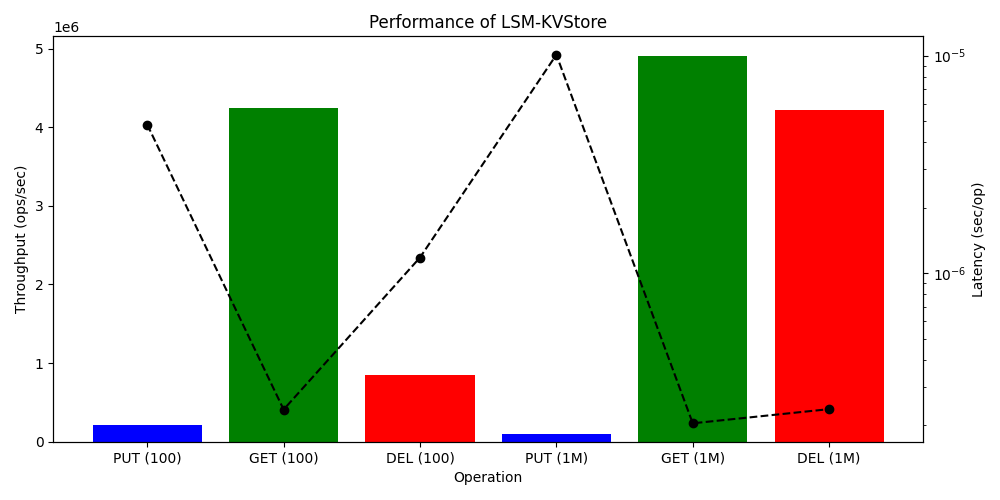
\includegraphics[width=0.9\textwidth]{Figure_1.png}
				\caption{实验数据图(三种操作的吞吐量和时延)}
				\label{fig:performance1}
			\end{figure}
			
		
		由实验结果可以得到:
        \begin{enumerate}
		\item PUT 操作性能分析:PUT 操作的吞吐量从 100 组测试的 207,307 ops/sec 降低到 1,000,000 组测试的 98,966 ops/sec,可能原因是数据规模变大,触发 \texttt{Compaction} 影响写入速度。在 100 组数据时,写入只涉及内存;而 1,000,000 组数据后,写入速度受到磁盘 I/O 限制。
		\item GET 操作性能分析:GET 操作的吞吐量从 100 组测试的 4,245,560 ops/sec 提升到 1,000,000 组测试的 4,909,830 ops/sec,和预期相反,可能原因是索引和 Bloom Filter 的优化使得查询比跳表更快,合并后数据更集中,从而加快了查询速度。
		\item DELETE 操作性能分析:DELETE 操作的吞吐量从 100 组测试的 845,266 ops/sec 提升到 1,000,000 组测试的 4,212,730 ops/sec,也与预期相反,可能原因 DELETE 操作只是在 GET 的基础上打上 DEL 标记,在 \texttt{Compaction} 过程中,标记删除的数据会被彻底清理。受益于 GET 查询效率的提升,删除操作也变快了。
		\end{enumerate}


	\section{结论}
	\hspace{2em}实验结果表明,PUT 操作在数据量增加后,吞吐量下降了约 52\%,主要受到 \texttt{Compaction} 额外 I/O 限制,硬盘存储的速度比较慢;GET 操作吞吐量在数据规模扩大后 反而提升了约 15\%,表明 \texttt{Compaction} 通过索引和 Bloom Filter 优化,提升了查询效率。DELETE 操作吞吐量提升了 近 5 倍,表明 \texttt{Compaction} 通过存入删除标记、减少查询负担,使得删除操作的效率明显提高。
	
	\texttt{Compaction} 在提高查询和删除性能的同时,降低了写入吞吐量。因此,在实际应用中,LSM Tree 适用于写入相对较少,但查询和删除操作较频繁的场景,例如日志存储、搜索引擎索引等。
	
	\section{致谢}
	
	\hspace{2em}在本项目的过程中,我得到了许多人的帮助与支持,在此向他们表示诚挚的感谢。
	
	我要感谢我的AI助手(ChatGPT),它为我提供了很多绘图代码上的帮助,帮助我高效地解决了问题。
	
	
	\section{其他和建议}
	\subsection{其他优化}
	\hspace{2em} 本 project 中的 \texttt{Compaction} 函数实现时使用循环次数较多,对性能损耗影响较大,可以进一步优化。
	
	\subsection{吐槽}
	 	\hspace{2em}一跑跑15分钟的代码总是让人怀疑是不是死循环了...
	
	%\hspace{2em}感觉随机种子的影响力很大,取5组数据取平均值的时候出现了反常趋势,如图~\ref{fig:abnormal}。
	%	\begin{figure}[H]
		%	\centering
		%	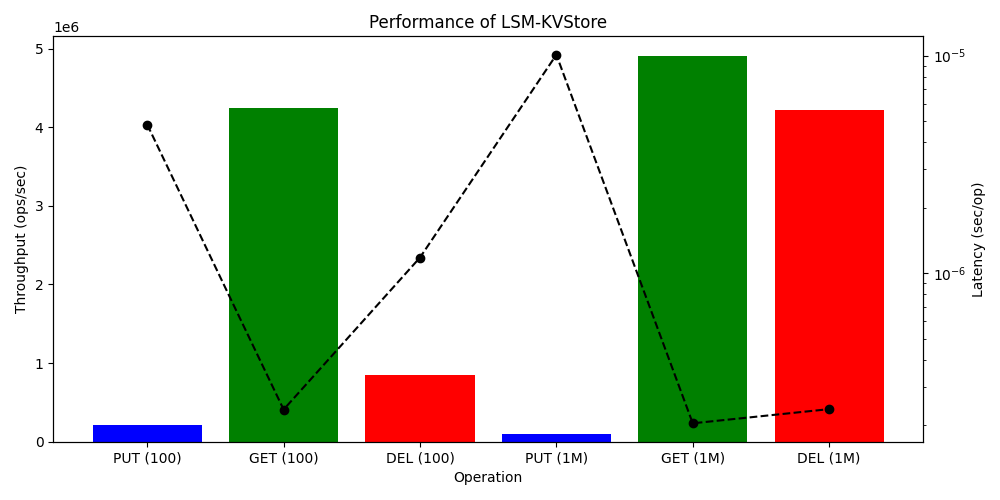
\includegraphics[width=0.9\textwidth]{Figure_1.png}
		%	\caption{反常数据}
		%	\label{fig:abnormal}
		%\end{figure}
	
	
	
	%	这是一个对图片的引用, 图~\ref{fig:universe},以及参考文献~\cite{adams1995hitchhiker}。
	%
	%	\begin{figure}[h!]
		%	\centering
		%	\includegraphics[width=0.5\textwidth]{universe}
		%	\caption{The Universe}
		%	\label{fig:universe}
	%\end{figure}
	
	%\section{代码}
	%\subsection{run\_experiments.sh}
	%\lstinputlisting[language=Bash]{run_experiments.sh}
	%\subsection{plot\_results.py}
	%\lstinputlisting[language=python]{plot_results.py}
	
	\nocite{*}
	%\bibliography{references}
	
\end{document}
